\chapter{Introduction}


\section{Motivation and Background}

% Autonomous Vehicle

An autonomous vehicle has great potential to improve driving safety, comfort and efficiency and can be widely applied in a variety of fields, such as road transportation, agriculture, planetary exploration, military purpose and so on \cite {WANG2015727}. The past three decades have witnessed the rapid development of autonomous vehicle technologies, which have attracted considerable interest and efforts from academia, industry, and governments. Particularly in the past decade, contributing to significant advances in sensing, computer technologies, and artificial intelligence, the autonomous vehicle has become an extraordinarily active research field. During this period, several well-known projects and competitions for autonomous vehicles have already exhibited autonomous vehicles' great potentials in the areas ranging from unstructured environments to the on-road driving environments \cite{AutonomousStructured} \cite{DrivingUrban2008}.

% Highway Driving

Complex functions like highly autonomous driving with combined longitudinal and lateral control will definitely appear first on highways, since traffic is more predictable and relatively safe there (one-way traffic only, quality road with relative wide lanes, side protections, good visible lane markings, no pedestrians or cyclists, etc.). As highways are the best places to introduce hands-free driving at higher speeds, one could expect a production vehicle equipped with a temporary autopilot or in other words autonomous highway driving assist function as soon as the end of this decade. 

Autonomous highway driving means the autonomous control of the complex driving tasks of highway driving, like driving at a safe speed selected by the driver, changing lanes or overtaking front vehicles depending on the traffic circumstances, automatically reducing speed as necessary or stopping the vehicle in the right most lane in case of an emergency. Japanese Toyota Motor have already demonstrated their advanced highway driving support system prototype in real traffic operation. The two vehicles  communicate each other, keeping their lane and following the preceding vehicle to maintain a safety distance \cite{Nissan2013}.

% Simulator
An important aspect in developing an autonomous driving system is the development of a simulator. To get to mass production, autonomous vehicles must drive 10 billion kilometers for proof of concept. With 100 vehicles driving 24 hours seven days a week , this would still mean 225 years of driving. Simulators can accelerate that and reduce costs. Both Uber and Waymo recently gave a glimpse into the workings of their simulators, with which they ``drive'' billions kilometer per year.

% Adaptive Cruise Control

In this thesis, we are aiming for developing an autonomous driving system allowing the vehicle to smartly choose the driving behaviors, such as adjusting the speed and changing the lane. For the longitudinal motion, Adaptive cruise control (ACC), a radar-based system, is to enhance driving comfort and convenience by relieving the need to continually adjust the speed to match that of a preceding vehicle. The system slows down when it approaches a vehicle with a lower speed, and the system increases the speed to the level of speed previously set when the vehicle upfront accelerates or disappears (e.g., by changing lanes) \cite{ACC2002}. As for the lateral motion, Autonomous lane control system, relying on position sensors, identifies a current lane where the vehicle is located, provides instructions to the steering system and speed control system to maneuver the vehicle in either the lane-keeping mode or the lane-changing mode \cite{LaneControl2012}. Traditional methods have proved the reliability in several cases though the use is still quite limited and only for expected scenarios. While, currently, artificial intelligence especially deep reinforcement learning is aggressively expanding the border of human's imagination and machine's autonomy. Thus, a new learning based adaptive cruise and lane control system is proposed for autonomous vehicles with the help of deep reinforcement learning.

\section{Literation Review}

The past few years have seen many breakthroughs using reinforcement learning (RL). The company DeepMind combined deep learning with reinforcement learning to achieve above-human results on a multitude of Atari games and, in March 2016, defeated Go champion Le Sedol four games to one. Though RL is currently excelling in many game environments, it is a novel way to solve problems that require optimal decisions and efficiency, and will surely play a part in machine intelligence to come.

% The rise of Deep Q Learning

Google's DeepMind published its famous paper Playing Atari with Deep Reinforcement Learning \cite {Mnih2015AtariNature}, in which they introduced a new algorithm called Deep Q Network (DQN for short) in 2013. It demonstrated how an AI agent can learn to play games by just observing the screen without any prior information about those games. The result turned out to be pretty impressive. This paper opened the era of what is called ``deep reinforcement learning'', a mix of deep learning and reinforcement learning.

% Reinforcement Learning
Reinforcement Learning is a type of machine learning that allows you to create AI agents that learn from the environment by interacting with it. Just like how we learn to ride a bicycle, this kind of AI learns by trial and error. As seen in Fig. \ref {fig:deepmind}, the robot represents the AI agent, which acts on the environment. After each action, the agent receives the feedback. The feedback consists of the reward and next state of the environment. The reward is usually defined by a human. If we use the analogy of the bicycle, we can define reward as the distance from the original starting point.

\begin{figure}[h] 
\centering
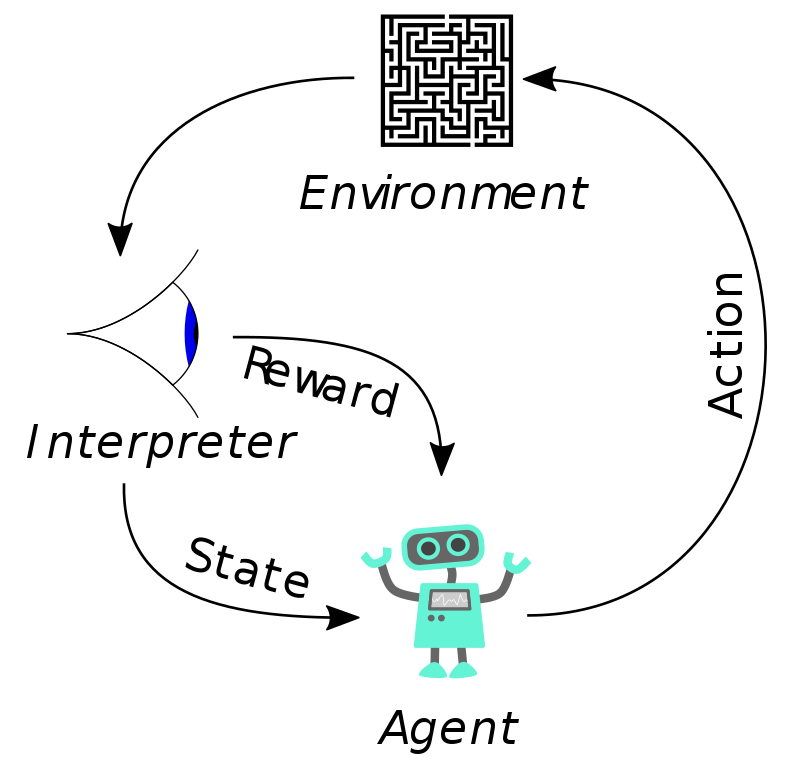
\includegraphics[width=0.8\textwidth]{figs/ch1/Reinforcement_learning_diagram}
\caption{How an agent interacts with the environment.}
\label{fig:deepmind}
\end{figure}

Standard model-based methods for robotic manipulation might involve estimating the physical properties of the environment, and then solving for the controls based on the known laws of physics \cite{OK-Robot-1987} \cite{Predictive2014} \cite{PlanningFramework2012}. This approach has been applied to a range of problems. However, estimating and simulating all of the details of the physical environment is exceedingly difficult, particularly for previously unseen objects, and is arguably unnecessary if the end goal is only to find the desired controls. For example, simple rules for adjusting motion, such as increasing force when an object is not moving fast enough, or the gaze heuristic \cite{FieldersNature2003}, can be used to robustly perform visuomotor control without an overcomplete representation of the physical world and complex simulation calculations. A learning based framework could avoid the detailed and complex modeling associated with the fully model-based approach.

Several works have used deep neural networks to process images and represent policies for robotic control, initially for driving tasks \cite{AutonomousLand1989} \cite{LongrangeVision2009}, later for robotic soccer \cite{RobotSoccer2009}, and most recently for robotic grasping \cite{Grasp2016} \cite{RooticGrasping2016} and manipulation \cite{Visuomotor2016}. Although these model-free methods can learn highly specialized and proficient behaviors, they recover a task-specific policy rather than a flexible model that can be applied to a wide variety of different tasks. The high dimensionality of image observations presents a substantial challenge to model-based approaches, which have been most successful for low-dimensional non-visual tasks \cite{PolicySearch2011} such as helicopter control \cite{HeliNg2007}, locomotion \cite{Trajectory2012}, and robotic cutting \cite{Deepmpc2015}. Nevertheless, some works have considered modeling high-dimensional images for object interaction. For example, Boots et al. \cite{Predictive2014} learn a predictive model of RGB-D images of a robot arm moving in free space.

% ACC

A lot of related work has been done in recent years in the design of ACC systems. Regarding the vehicle-following controller, Hallouzi et al. [8] did some research as part of the CarTalk 2000 project. These authors worked on the design of a longitudinal Cooprated-ACC controller based on vehicle-to-vehicle communication. They showed that inter-vehicle communication can help reduce instability of a platoon of vehicles. In the same vein, Naranjo and his colleague [14] worked on designing a longitudinal controller based on fuzzy logic. Their approach is similar to what we did with reinforcement learning for our low-level controller. Forbes has presented a longitudinal reinforcement learning controller [5] and compared it to a hand-coded following controller. He showed that the hand-coded controller is more precise than its RL controller but less adaptable in some situations.

% Lane Control

Regarding the reinforcement learning in a lane control problem, Unsal, Kachroo and Bay \cite{CACC1999} have used multiple stochastic learning automata to control the longitudinal and lateral path of a vehicle. In his work, Pendrith \cite{DistributedRL-Traffic2000} presented a distributed variant of Q-Learning (DQL) applied to lane change advisory system, that is close to the problem described in this thesis. His approach uses a local perspective representation state which represents the relative velocities of the vehicles around. Consequently, this representation state is closely related to our state representation. 

On the other hand, our high level controller model is similar to Partially Observable Stochastic Games (POSG). This model formalizes theoretically the observations for each agent. The resolution of this kind of games has been studied by Emery-Montermerlo \cite{GameControl2005}. This resolution is an approximation using Bayesian games. However, this solution is still based on the model of the environment, unlike our approach which does not take into account this information explicitly since we assume that the environment is unknown. Concerning the space search reduction, Sparse Cooperative Q-Learning \cite{Sparse2004} allows agents to coordinate their actions only on predefined set of states. In the other states, agents learn without knowing the existence of the other agents.

\section{Thesis Outline}

The goal of this thesis is to develop a learning framework for the autonomous driving system. This section will present the chapters and subsections of this thesis and provide a brief summary of those sections.

Chapter 2 details the stack architecture of the simulating environment and the integration of the simulating tools.

\begin{itemize}
\item \textbf {Section 2.1 ROS:} A general introduction of Robotic Operating System (ROS).
\item \textbf {Section 2.2 Gazebo:} A general introduction of Gazebo, a robot dynamic simulator.
\item \textbf {Section 2.3 OpenAI-Gym:} A general introduction of OpenAI-Gym, an open source AI playground and environment builder.
\item \textbf {Section 2.4 Vehicle Model:} A close-to-reality vehicle model.
\end{itemize}

Chapter 3 dives into the autonomous driving system. Chapter 3 is laid out as follows:

\begin{itemize}
\item \textbf {Section 3.1 Behavior Planning:} 
\item \textbf {Section 3.2 Path Planning:}
\item \textbf {Section 3.3 Path Flowing:}
\item \textbf {Section 3.4 Drive By Wire:} 
\end{itemize}

Chapter 4 describes the core algorithm in the framework, namely Deep Q-Learning. Chapter 4 is a follows:

\begin{itemize}
\item \textbf {Section 4.1 Architecture:} 
\item \textbf {Section 4.2 Reinforcement Learning for Longitudinal Motion:}
\item \textbf {Section 4.3 Reinforcement Learning for Lateral Motion:}
\item \textbf {Section 4.4 Q Learning:} 
\item \textbf {Section 4.5 Policy Representation}
\item \textbf {Section 4.6 Deep Neural Network}
\end{itemize}

Chapter 5 displays the experiment results in some basic scenarios. Chapter 5 sections are as follows:

\begin{itemize}
\item \textbf {Section 5.1 Simulation Setup:} 
\item \textbf {Section 5.2 Training for Longitudinal Motion:}
\item \textbf {Section 5.3 Training for Lateral Motion:}
\item \textbf {Section 5.4 Training for Combined Motion:} 
\end{itemize}

Chapter 6 contains the conclusion. Chapter 6 sections are as follows:

\begin{itemize}
\item \textbf {Section 6.1 Free-Form Visualization:} 
\item \textbf {Section 6.2 Analysis:} 
\item \textbf {Section 6.2 Reflection:} 
\end{itemize}

Chapter 7 indicates several promising areas for future work. 

%%%%%%%%%%%%%%%%%%%%%%%%%%%%%%%%%%%%%%%%%%%%%%%%%%%%%%%%%%%%%%%%%%%%%%%%%%%%%%%%%%%%%%%%%%%%%%%%%%%%



%\bibliographystyle{plainnat}
%\markright{\textit{Bibliography}}
%\renewcommand{\chaptername}{}
%x\bibliography{KL-Thesis}

\vfill

